\documentclass[%twoside,                   								  % Impressão em frente e verso 	        oneside,                   								  % Impressão apenas frente
openany
]{configuracoes/ifbaiano-abntex2}

% INCLUI ARQUIVOS DE  CONFIGURAÇÕES----------------------------------------
% Instituto Federal de Educação, Ciência e Tecnologia Baiano - Campus Guanambi
% 
% Modelo para Trabalho de Conclusão de Curso em LaTeX
% Superior de Análise e Desenvolvimento de Sistemas
% Alterado por: Dr. Naidson Clayr Santos Ferreira
%
% ----------------------------------------------------------------------- %
% Arquivo: pacotes.tex
% ----------------------------------------------------------------------- %

% REFERÊNCIAS------------------------------------------------------------------
\usepackage[%
    alf,
    abnt-emphasize=bf,
    bibjustif,
    recuo=0cm,
    abnt-url-package=url,       % Utiliza o pacote url
    abnt-refinfo=yes,           % Utiliza o estilo bibliográfico abnt-refinfo
    abnt-etal-cite=3,
    abnt-etal-list=3,
    abnt-thesis-year=final
]{abntex2cite}                  % Configura as citações bibliográficas conforme a norma ABNT

% PACOTES----------------------------------------------------------------------
\usepackage{amssymb}
% símbolos matemáticos

% Codificação do documento
\usepackage[utf8]{inputenc}
     
% Seleção de código de fonte                           
\usepackage[T1]{fontenc}
                                    
% Réguas horizontais em tabelas
\usepackage{booktabs}

% Controle das cores                                       
\usepackage{color, colortbl}   

% Necessário para tabelas/figuras em ambiente multi-colunas
\usepackage{float}

% Inclusão de gráficos e figuras
\usepackage{graphicx}

% Uso de vírgulas em expressões matemáticas
\usepackage{icomma}

% Indenta o primeiro parágrafo de cada seção
\usepackage{indentfirst}

% Melhora a justificação do documento
\usepackage{microtype}

% Permite tabelas com múltiplas linhas e colunas
\usepackage{multirow, array}

% Permite subnumeração de equações
\usepackage{subeqnarray}

% Para encontrar última página do documento                                    
\usepackage{lastpage} 

% Permite apresentar texto tal como escrito no documento, ainda que sejam comandos Latex                                      
\usepackage{verbatim}

% Fontes e símbolos matemáticos                                       
\usepackage{amsfonts, amssymb, amsmath}
             
% Permite escrever algoritmos em português                     
\usepackage[algoruled, portuguese]{algorithm2e}
             
% Usa a fonte Helvetica             
%\usepackage[scaled]{helvet}
 
% Usa a fonte Times                                
\usepackage{times}
                                         
% Usa a fonte Palatino
%\usepackage{palatino}

% Usa a fonte Latin Modern                                      
%\usepackage{lmodern}

% Mantém as notas de rodapé sempre na mesma posição                                       
\usepackage[bottom]{footmisc}
        
% Fontes de alta qualidade                              
\usepackage{ae, aecompl}

% Símbolos matemáticos                                    
\usepackage{latexsym}

% Permite páginas em modo "paisagem"                                       
\usepackage{lscape}
 
% Dispor imagens em parágrafos                                         
%\usepackage{picinpar}                                      

%Tabela Colorida
\usepackage{colortbl}
\usepackage{xcolor}

%Tabelas Longas
\usepackage{longtable}
\usepackage[graphicx]{realboxes}
%\usepackage{scalefnt}                                      % Permite redimensionar tamanho da fonte
%\usepackage{subfig}                                        % Posicionamento de figuras
%\usepackage{upgreek}                                       % Fonte letras gregas

% Redefine a fonte para uma fonte similar a Arial (fonte Helvetica)
%\renewcommand*\familydefault{\sfdefault}
										  % Comando para Configurações de Pacote
% Instituto Federal de Educação, Ciência e Tecnologia Baiano - Campus Guanambi
% 
% Modelo para Trabalho de Conclusão de Curso em LaTeX
% Superior de Análise e Desenvolvimento de Sistemas
% Alterado por: Dr. Naidson Clayr Santos Ferreira
%
% ----------------------------------------------------------------------- %
% Arquivo: configuracoes-pdf.tex
% ----------------------------------------------------------------------- %

% CONFIGURAÇÕES DE APARÊNCIA DO PDF FINAL--------------------------------------
\makeatletter
\hypersetup{%
    portuguese,
    colorlinks=true,   % true: "links" coloridos; false: "links" em caixas de texto
    linkcolor=black,    % Define cor dos "links" internos
    citecolor=black,    % Define cor dos "links" para as referências bibliográficas
    filecolor=black,    % Define cor dos "links" para arquivos
    urlcolor=black,     % Define a cor dos "hiperlinks"
    breaklinks=true,
    pdftitle={\@title},
    pdfauthor={\@author},
    pdfkeywords={abnt, latex, abntex, abntex2}
}
\makeatother

% ALTERA O ASPECTO DA COR AZUL--------------------------------------------------
\definecolor{blue}{RGB}{41,5,195}

% REDEFINIÇÃO DE LABELS---------------------------------------------------------
\renewcommand{\algorithmautorefname}{Algoritmo}
\def\equationautorefname~#1\null{Equa\c c\~ao~(#1)\null}

% CRIA ÍNDICE REMISSIVO---------------------------------------------------------
\makeindex

% HIFENIZAÇÃO DE PALAVRAS QUE NÃO ESTÃO NO DICIONÁRIO---------------------------
\hyphenation{%
    qua-dros-cha-ve
    Kat-sa-gge-los
}
								  % Comando para Configurações de PDF


% INCLUI ARQUIVOS DO TRABALHO DE CONCLUSÃO DE CURSO (PRÉ-TEXTUAIS, TEXTUAIS, PÓS-TEXTUAIS)-----------------------

% INSERE CAPA E FOLHA DE ROSTO
% Instituto Federal de Educação, Ciência e Tecnologia Baiano - Campus Guanambi
% 
% Modelo para Trabalho de Conclusão de Curso em LaTeX
% Superior de Análise e Desenvolvimento de Sistemas
% Alterado por: Dr. Naidson Clayr Santos Ferreira and Msc. Tiago Nogueira
%
% ----------------------------------------------------------------------- %
% Arquivo: capa.tex
% ----------------------------------------------------------------------- %

% CAPA---------------------------------------------------------------------------------------------------

% ORIENTAÇÕES GERAIS-------------------------------------------------------------------------------------
% Caso algum dos campos não se aplique ao seu trabalho, como por exemplo,
% se não houve coorientador, apenas deixe vazio.
% Exemplos: 
%\coorientador{Coloque o Nome do Coorientador}
%\departamento{Instituição do Coorientador}

% DADOS DO TRABALHO--------------------------------------------------------------------------------------
\titulo{Sistema de Comando e Controle no apoio a decisão: um breve estudo de caso.}
\titleabstract{Educational Data Mining for Performance Forecasting and Student Evasion in Introductory Algorithm Disciplines}
\autor{José Gustavo Sousa Peres e Nelson dos Santos Luz}
\autorcitacao{PERES, José, LUZ, Nelson} % Sobrenome em maiúsculo
\local{Brasília}
\data{2019}

% NATUREZA DO TRABALHO-----------------------------------------------------------------------------------
% Opções: 
% - Trabalho de Conclusão de Curso (se for Graduação)
% - Dissertação (se for Mestrado)
% - Tese (se for Doutorado)
% - Projeto de Qualificação (se for Mestrado ou Doutorado)
\projeto{Trabalho de Conclusão de Curso}

% TÍTULO ACADÊMICO---------------------------------------------------------------------------------------
% Opções:
% - Bacharel ou Tecnólogo (Se a natureza for Trabalho de Conclusão de Curso)
% - Mestre (Se a natureza for Dissertação)
% - Doutor (Se a natureza for Tese)
% - Mestre ou Doutor (Se a natureza for Projeto de Qualificação)
\tituloAcademico{Tecnólogo em Gestão Militar}

% ÁREA DE CONCENTRAÇÃO E LINHA DE PESQUISA---------------------------------------------------------------
% Se a natureza for Trabalho de Conclusão de Curso, deixe ambos os campos vazios
% Se for programa de Pós-graduação, indique a área de concentração e a linha de pesquisa
\areaconcentracao{Análise de Sistemas de Apoio à Decisão}
\linhapesquisa{Comando e Controle}

% DADOS DA INSTITUIÇÃO-----------------------------------------------------------------------------------
% Se a natureza for Trabalho de Conclusão de Curso, coloque o nome do curso de graduação em "programa"
% Formato para o logo da Instituição: \logoinstituicao{<escala>}{<caminho/nome do arquivo>}
\mec{Exército Brasileiro}
\setec{DECEx - DETMil}
\instituicao{Escola de Instrução Especializada}
%\departamento{Coint - Tecnologia em Sistemas para Internet}
\programa{Curso de Habilitação ao Quadro Auxiliar de Oficiais}
% \logoinstituicao{4cm}{Figuras/logoIsie.png} 

% DADOS DOS ORIENTADORES---------------------------------------------------------------------------------
\orientador{Carlos Henrique da Costa}
%\orientador[Orientadora:]{Nome da orientadora}
\instOrientador{Centro de Desenvolvimento de Sistema}

\coorientador{}
%\coorientador[Coorientadora:]{Nome da coorientadora}
\instCoorientador{}

% Instituto Federal de Educação, Ciência e Tecnologia Baiano - Campus Guanambi
% 
% Modelo para Trabalho de Conclusão de Curso em LaTeX
% Superior de Análise e Desenvolvimento de Sistemas
% Alterado por: Dr. Naidson Clayr Santos Ferreira
%
% ----------------------------------------------------------------------- %
% Arquivo: folha-rosto.tex
% ----------------------------------------------------------------------- %

% FOLHA DE ROSTO--------------------------------------------------------------------------------------------------
% TRABALHO DE CONCLUSÃO DE CURSO
 \preambulo{{\imprimirprojeto} apresentado a {\imprimirinstituicao} ligado ao {\imprimirmec}, como requisito parcial do {\imprimirprograma} para a obtenção do título de {\imprimirtituloAcademico}.}

% DISSERTAÇÃO DE MESTRADO
% \preambulo{{\imprimirprojeto} apresentada ao Programa de \mbox{Pós-graduação} da {\imprimirinstituicao}, como requisito parcial para obtenção do título de {\imprimirtituloAcademico}.}

% TESE DE DOUTORADO
% \preambulo{{\imprimirprojeto} apresentada ao Programa de \mbox{Pós-graduação} da {\imprimirinstituicao}, como requisito parcial para a obtenção do título de {\imprimirtituloAcademico}.}

% PROJETO DE QUALIFICAÇÃO DE MESTRADO OU DOUTORADO
%\preambulo{{\imprimirprojeto} apresentado ao Programa de \mbox{Pós-graduação} da {\imprimirinstituicao}, como requisito parcial para a obtenção do título de {\imprimirtituloAcademico}.}

% OBSERVAÇÕES-----------------------------------------------------------------------------------------------------------
% Altere este arquivo APENAS comentando as linhas que não se aplicam ao tipo de trabalho acadêmico desejado.



\begin{document}

\pretextual
\imprimircapa                        								   % Comando para imprimir Capa}}
\imprimirfolhaderosto{}                 								   % Comando para imprimir Folha de rosto
%\imprimirfolhadeaprovacao												   % Comando para imprimir Folha de Aprovação

% INSERE ELEMENTOS PRÉ-TEXTUAIS
%% Instituto Federal de Educação, Ciência e Tecnologia Baiano - Campus Guanambi
% 
% Modelo para Trabalho de Conclusão de Curso em LaTeX
% Superior de Análise e Desenvolvimento de Sistemas
% Alterado por: Dr. Naidson Clayr Santos Ferreira
%
% ----------------------------------------------------------------------- %
% Arquivo: folha-aprovacao.tex
% ----------------------------------------------------------------------- %


\begin{folhadeaprovacao}
	\begin{center}
		
		{\ABNTEXchapterfont\large\MakeUppercase{\imprimirautor}}
		
		\vspace{30pt}
		
		\vspace*{\fill}\vspace*{\fill}
		
		\begin{center}
			
			{\ABNTEXchapterfont\bfseries\large\MakeUppercase{\imprimirtitulo}}
			
		\end{center}
		
		\vspace*{\fill}
		
		\hspace{.45\textwidth}
		
		\begin{flushright}
			\begin{minipage}{.5\textwidth}
				\imprimirpreambulo	
			\end{minipage}
		\end{flushright}
		
		\vspace*{\fill}
		
	\end{center}
	
	\vspace{10pt}
	
	\begin{flushleft}
		
	{\bfseries Trabalho aprovado. \imprimirlocal, 24 de Novembro de 2017}
		
	\end{flushleft}
	
	\vspace{10pt}
	
	\begin{flushleft}
		BANCA EXAMINADORA:
		
		\vspace{18pt}
		
		\rule{7cm}{.1mm} \\
		{Título. Nome do Professor \\ Nome da Instituição} \\ [1.0cm]
		\rule{7cm}{.1mm} \\
		{Título. Nome do Professor \\ Nome da Instituição} \\ [1.0cm]
		
	
	\end{flushleft}
	
	
	\begin{center}
		
		{Título. Nome do orientador \\ Orientador} \\ [1.0cm]
		{Título. Nome do Coorientador \\ Coorientador} \\[.6cm]
		
	\end{center}
	
	\begin{center}
		
		\vspace*{0.5cm}
		
		{\MakeUppercase\imprimirlocal}
		
		\par
		
		{\MakeUppercase\imprimirdata}
		
		\vspace*{1cm}
		
	\end{center}
\end{folhadeaprovacao}

% -----------------------------------------------------------------------------
% Este documento foi mantido apenas para preservar a paginação do trabalho
% acadêmico final, após a inserção da folha de aprovação fornecida
% -----------------------------------------------------------------------------

%% Instituto Federal de Educação, Ciência e Tecnologia Baiano - Campus Guanambi
% 
% Modelo para Trabalho de Conclusão de Curso em LaTeX
% Superior de Análise e Desenvolvimento de Sistemas
% Alterado por: Dr. Naidson Clayr Santos Ferreira
%
% ----------------------------------------------------------------------- %
% Arquivo: dedicatoria.tex
% ----------------------------------------------------------------------- %

% DEDICATÓRIA------------------------------------------------------------------

\renewcommand{\dedicatorianame}{DEDICATÓRIA}

\begin{dedicatoria}

Altere este texto inserindo a dedicatória do seu trabalho. 

\end{dedicatoria}
          			   	       % Dedicatória
%% Instituto Federal de Educação, Ciência e Tecnologia Baiano - Campus Guanambi
% 
% Modelo para Trabalho de Conclusão de Curso em LaTeX
% Superior de Análise e Desenvolvimento de Sistemas
% Alterado por: Dr. Naidson Clayr Santos Ferreira
%
% ----------------------------------------------------------------------- %
% Arquivo: agradecimentos.tex
% ----------------------------------------------------------------------- %

% AGRADECIMENTOS---------------------------------------------------------------

\begin{agradecimentos}[AGRADECIMENTOS]

Edite e coloque aqui os agradecimentos às pessoas e/ou instituições que contribuíram para a realização do trabalho.

É obrigatório o agradecimento às instituições de fomento à pesquisa que financiaram total ou parcialmente o trabalho, inclusive no que diz respeito à concessão de bolsas.

\end{agradecimentos}
        			       % Agradecimentos
%% Instituto Federal de Educação, Ciência e Tecnologia Baiano - Campus Guanambi
% 
% Modelo para Trabalho de Conclusão de Curso em LaTeX
% Superior de Análise e Desenvolvimento de Sistemas
% Alterado por: Dr. Naidson Clayr Santos Ferreira
%
% ----------------------------------------------------------------------- %
% Arquivo: epigrafe.tex
% ----------------------------------------------------------------------- %

% EPÍGRAFE---------------------------------------------------------------------

\renewcommand{\epigraphname}{EPÍGRAFE}

\begin{epigrafe}

\textit{...Isto é água... Isto é água. (WALLACE, David Foster, 2005).}

\end{epigrafe}

% OBSERVAÇÕES------------------------------------------------------------------
% Altere o texto para inserir a epígrafe do seu trabalho
              			       % Epígrafe
% Instituto Federal de Educação, Ciência e Tecnologia Baiano - Campus Guanambi
% 
% Modelo para Trabalho de Conclusão de Curso em LaTeX
% Superior de Análise e Desenvolvimento de Sistemas
% Alterado por: Dr. Naidson Clayr Santos Ferreira
%
% ----------------------------------------------------------------------- %
% Arquivo: resumo.tex
% ----------------------------------------------------------------------- %

% RESUMO--------------------------------------------------------------------------------

\begin{resumo}[RESUMO]
\begin{SingleSpacing}

% Não altere esta seção do texto--------------------------------------------------------
\imprimirautorcitacao. \imprimirtitulo. \imprimirdata. \pageref {LastPage} f. \imprimirprojeto\ – \imprimirprograma, \imprimirinstituicao. \imprimirlocal, \imprimirdata.\\
%---------------------------------------------------------------------------------------

Este trabalho apresenta um estudo sobre o Pacificador, o sistema de comando e controle desenvolvido pelo Exército, que tem como principal objetivo a garantia do sucesso das mais variadas operações desenvolvidas pelo Exército e apoiadas por este sistema. 
Na seção 2 realizaremos a definição de Comando e Controle, abordando de forma separada tanto o Comando como o Controle, suas características e os fatores determinantes no sucesso de uma operação. Falaremos também sobre os componentes imprescindíveis do Comando e Controle e suas interdependências.
Abordaremos na seção 3 o Sistema de Comando e Controle, sua principal missão, as categorias de informações mais importantes, funções básicas de um sistema C2, os cinco subconjuntos básicos para o sistema C2, a importância do recurso humano bem treinado para realizar as entradas fidedignas no sistema e a importância da computação no uso dos sistemas de Comando e Controle.
Na próxima seção apresentaremos as principais funcionalidades do Sistema Pacificador Web, quais órgãos do governo utilizam-no e em quais grandes eventos o sistema foi utilizado como ferramenta de comando e controle, bem como suas especificidades que foram determinantes para o sucesso daqueles eventos. Também falaremos sobre o impacto da mobilidade ou da falta dela para bom cumprimento da missão pelos agentes, o que é determinante para o pacificador.
Na última seção, realizaremos a análise estatística do uso do Sistema Pacificador Web pelos oito Comandos Militares de Área (C Mil A), iniciando pela distribuição e frequência de Centro de Operações pelos diversos C Mil A, distribuição de frequência de número de Agentes por cada grande comando, quantidade de Incidentes, Ações e Relatos nos diversos Comandos Militares e por último faremos uma conclusão da análise desses dados.
\\

\textbf{Palavras-chave}: comando e controle, grandes eventos, sistema de comando e controle, Pacificador.

\end{SingleSpacing}
\end{resumo}

% OBSERVAÇÕES---------------------------------------------------------------------------
% Altere o texto inserindo o Resumo do seu trabalho.
% Escolha de 3 a 5 palavras ou termos que descrevam bem o seu trabalho 
             			           % Resumo em Português
%% Instituto Federal de Educação, Ciência e Tecnologia Baiano - Campus Guanambi
% 
% Modelo para Trabalho de Conclusão de Curso em LaTeX
% Superior de Análise e Desenvolvimento de Sistemas
% Alterado por: Dr. Naidson Clayr Santos Ferreira
%
% ----------------------------------------------------------------------- %
% Arquivo: abstract.tex
% ----------------------------------------------------------------------- %

% ABSTRACT--------------------------------------------------------------------------------

\begin{resumo}[ABSTRACT]
\begin{SingleSpacing}

% Não altere esta seção do texto--------------------------------------------------------
\imprimirautorcitacao. \imprimirtitleabstract. \imprimirdata. \pageref {LastPage} f. \imprimirprojeto\ – \imprimirprograma, \imprimirinstituicao. \imprimirlocal, \imprimirdata.\\
%---------------------------------------------------------------------------------------

This work presents a study with the use of data mining focused on the educational context, in higher education courses, where there is a high number of students who fail in the curricular components of programming. The need for its realization arose from the observation of an unsatisfactory student performance in relation to the disciplines of algorithm and data structure. In order to do so, we chose the use of data from students enrolled in a public institution of higher learning, to be collected and analyzed using Support Vector Machine algorithms and processed with the WEKA tool, in order to create regression models capable of both pointing out evasion risks and predicting the possible causes of the high number of failures in such disciplines.\\

\textbf{Keywords}:Educational Data Mining. School Evasion. Support Vector Machine.

\end{SingleSpacing}
\end{resumo}

% OBSERVAÇÕES---------------------------------------------------------------------------
% Altere o texto inserindo o Abstract do seu trabalho.
% Escolha de 3 a 5 palavras ou termos que descrevam bem o seu trabalho 
             		               % Resumo em Inglês
% % Instituto Federal de Educação, Ciência e Tecnologia Baiano - Campus Guanambi
% 
% Modelo para Trabalho de Conclusão de Curso em LaTeX
% Superior de Análise e Desenvolvimento de Sistemas
% Alterado por: Dr. Naidson Clayr Santos Ferreira
%
% ----------------------------------------------------------------------- %
% Arquivo: lista-figuras.tex
% ----------------------------------------------------------------------- %

% Lista de Figuras----------------------------------------------------------------

\pdfbookmark[0]{\listfigurename}{lof}
\listoffigures*
\cleardoublepage

% OBSERVAÇÕES---------------------------------------------------------------------
% Este arquivo não precisa de ser alterado, pois a lista é gerada automaticamente.
   % Lista de Figuras
%% Instituto Federal de Educação, Ciência e Tecnologia Baiano - Campus Guanambi
% 
% Modelo para Trabalho de Conclusão de Curso em LaTeX
% Superior de Análise e Desenvolvimento de Sistemas
% Alterado por: Dr. Naidson Clayr Santos Ferreira
%
% ----------------------------------------------------------------------- %
% Arquivo: lista-quadros.tex
% ----------------------------------------------------------------------- %

% LISTA DE QUADROS----------------------------------------------------------------

\renewcommand{\listofquadrosname}{LISTA DE QUADROS}

\pdfbookmark[0]{\listofquadrosname}{loq}
\listofquadros*
\cleardoublepage

% OBSERVAÇÕES---------------------------------------------------------------------
% Este arquivo não necessita de ser editado. A lista é gerada automaticamente.
   % Lista de Quadros
% % Instituto Federal de Educação, Ciência e Tecnologia Baiano - Campus Guanambi
% 
% Modelo para Trabalho de Conclusão de Curso em LaTeX
% Superior de Análise e Desenvolvimento de Sistemas
% Alterado por: Dr. Naidson Clayr Santos Ferreira
%
% ----------------------------------------------------------------------- %
% Arquivo: lista-tabelas.tex
% ----------------------------------------------------------------------- %

% LISTA DE TABELAS-------------------------------------------------------------

\pdfbookmark[0]{\listtablename}{lot}
\listoftables*
\cleardoublepage

% OBSERVAÇÕES-------------------------------------------------------------------
% Este arquivo não precisa ser alterado, pois a lista é gerada automaticamente.
         		       % Lista de Tabelas
%% Instituto Federal de Educação, Ciência e Tecnologia Baiano - Campus Guanambi
% 
% Modelo para Trabalho de Conclusão de Curso em LaTeX
% Superior de Análise e Desenvolvimento de Sistemas
% Alterado por: Dr. Naidson Clayr Santos Ferreira
%
% ----------------------------------------------------------------------- %
% Arquivo: lista-siglas.tex
% ----------------------------------------------------------------------- %

% LISTA DE ABREVIATURAS E SIGLAS----------------------------------------------------------

\begin{siglas}
    \item[ABNT] Associação Brasileira de Normas Técnicas
    \item[DECOM] Departamento de Computação
\end{siglas}

% OBSERVAÇÕES-----------------------------------------------------------------------------
% Altere a lista acima para definir os acrônimos e siglas utilizados neste trabalho
          		       % Lista de Abreviaturas e Siglas
%% Instituto Federal de Educação, Ciência e Tecnologia Baiano - Campus Guanambi
% 
% Modelo para Trabalho de Conclusão de Curso em LaTeX
% Superior de Análise e Desenvolvimento de Sistemas
% Alterado por: Dr. Naidson Clayr Santos Ferreira
%
% ----------------------------------------------------------------------- %
% Arquivo: lista-simbolos.tex
% ----------------------------------------------------------------------- %

% LISTA DE SÍMBOLOS------------------------------------------------------------

\begin{simbolos}
    \item[$ \Gamma $] Letra grega Gama
    \item[$ \lambda $] Comprimento de onda
    \item[$ \in $] Pertence
\end{simbolos}

% OBSERVAÇÕES-------------------------------------------------------------------
% Altere a lista acima para definir os símbolos utilizados no trabalho
        		       % Lista de Símbolos
%% Instituto Federal de Educação, Ciência e Tecnologia Baiano - Campus Guanambi
% 
% Modelo para Trabalho de Conclusão de Curso em LaTeX
% Superior de Análise e Desenvolvimento de Sistemas
% Alterado por: Dr. Naidson Clayr Santos Ferreira
%
% ----------------------------------------------------------------------- %
% Arquivo: lista-algoritmos.tex
% ----------------------------------------------------------------------- %

% LISTA DE ALGORITMOS----------------------------------------------------------

\newcommand{\algoritmoname}{Algoritmo}
\renewcommand{\listalgorithmcfname}{LISTA DE ALGORITMOS}

\floatname{algocf}{\algoritmoname}
\newlistof{listofalgoritmos}{loa}{\listalgoritmoname}
\newlistentry{algocf}{loa}{0}

\counterwithout{algocf}{chapter}
\renewcommand{\cftalgocfname}{\algoritmoname\space}
\renewcommand*{\cftalgocfaftersnum}{\hfill--\hfill}

\pdfbookmark[0]{\listalgorithmcfname}{loa}
\listofalgorithms
\cleardoublepage

% OBSERVAÇÕES------------------------------------------------------------------
% Este arquivo não precisa ser alterado, pois a lista é gerada automaticamente.
   % Lista de Algoritmos
% Instituto Federal de Educação, Ciência e Tecnologia Baiano - Campus Guanambi
% 
% Modelo para Trabalho de Conclusão de Curso em LaTeX
% Superior de Análise e Desenvolvimento de Sistemas
% Alterado por: Dr. Naidson Clayr Santos Ferreira
%
% ----------------------------------------------------------------------- %
% Arquivo: sumario.tex
% ----------------------------------------------------------------------- %

% SUMÁRIO----------------------------------------------------------------------

\renewcommand{\contentsname}{SUMÁRIO}

\pdfbookmark[0]{\contentsname}{toc}
\tableofcontents*
\cleardoublepage

% OBSERVAÇÕES-------------------------------------------------------------------
% Este arquivo não precisa ser alterado, pois o sumário é gerado automaticamente.
               			           % Sumário

\textual
% Instituto Federal de Educação, Ciência e Tecnologia Baiano - Campus Guanambi
% 
% Modelo para Trabalho de Conclusão de Curso em LaTeX
% Superior de Análise e Desenvolvimento de Sistemas
% Alterado por: Dr. Naidson Clayr Santos Ferreira
%
% ----------------------------------------------------------------------- %
% Arquivo: introducao.tex
% ----------------------------------------------------------------------- %

% INTRODUÇÃO-------------------------------------------------------------------

\chapter{INTRODUÇÃO}
% \hspace{1.5cm}
Devido ao permanente estado de prontidão do Exército Brasileiro (EB), para atender as demandas da defesa nacional buscando a garantia da lei e da ordem, desenvolvimento nacional e o bem-estar social. Segundo \cite{operacao2017}, com o advento das mudanças na sociedade e a crescente utilização de  tecnologia nas operações militares, as guerras têm experimentado alterações significativas ao longo dos tempos. Com as atuais estruturas geopolíticas na história dos conflitos temos o aumento da importância dos fatos militares e não militares na busca da resolução das conflagrações, através de recentes capacidades.

% \hspace{1.5cm}
Hoje mesmo com o advento tecnológico, nas suas diversas áreas, os conflitos convencionais, bem como as disputas de alta intensidade mantém suas condutas predominantes. Nos dias atuais o processo de decisão, sob uma ação de comando, deve ser realizada no momento adequado e com a maior brevidade possível. Neste contexto, é que os sistemas de Comando de Controle, em particular o Pacificador, tem a finalidade de ser uma fonte de apoio a decisão no conjunto das operações militares dentro de um plano ou ordem intentando cumprir uma atividade, tarefa, missão ou atribuição. 

% \hspace{1.5cm}
O objetivo deste trabalho, é realizar uma análise estatística do uso do Pacificador, um sistema de comando e controle desenvolvido pelo Centro de Desenvolvimento de Sistemas e utilizado por várias Organizações Militares (OM) do EB. O escopo desta análise será discorrer sobre quais são os incidentes mais comuns, média de tempo de resolução dos incidentes ao longo dos anos, quantas e quais as operações o sistema já apoiou, quantos usuários já utilizaram, quais e quantos Centros de Operações foram criados.

% \hspace{1.5cm}
A metodologia encontra-se dividida em três fases onde, na primeira fase, são coletados os dados do sistema, desde o momento de sua colocação em produção. Na segunda fase são analisados quais os dados poderão ser melhor comparados para que sejam geradas informações relevantes à pesquisa e, por fim, na terceira fase, são demonstradas as melhorias que o sistema trouxe à Força Terrestre e as possíveis melhorias que podem ser implementadas.

% \hspace*{1.5cm}
A execução da abordagem metodológica, apresentada nesta seção, servirá como forma de trabalhar os conceitos estudados no referencial teórico, bem como responder às questões levantadas durante a apresentação do problema e justificativa da pesquisa, além de alcançar os objetivos do trabalho.




        

\chapter{COMANDO E CONTROLE}

Segundo \cite{undestanding2006}, a função Comando e Controle não é um fim em si mesmo, porém é meio para consegui criar valores (ex: o rastreamento de uma operação. Basicamente, C2 é sobre evidenciar esforços sobre determinados números de entidades, sendo elas Organizações ou pessoas, recursos, tais como informação gerando assim algumas tarefas, objetivos e metas. A definição de Comando e Controle é  incompleta e potencialmente inútil a menos que venha a prover medidas existentes. 


Mesmo o C2 sendo necessário ele não é a garantia do sucesso da operações. Este sucesso tem dependência de vários outros fatores, incluindo a disponibilidade dos meios apropriados, suas capacidades operacionais e além dos inimigos e outras adversidades do Teatro de Operação. O êxito de Comando e Controle não pode ser definido pelo o sucesso nas missões, levando em conta que missão é uma ação de comando.
% Talvez tenha que recuar pois copie todo o texto do EB20-MC-10.205
A definição de Comando e Controle encontrada no Manual EB20-MC-10.205 é:
\begin{quote}
 Constitui-se  no  exercício  da  autoridade  e  da  direção que um comandante tem sobre as forças sob o próprio comando, para o cumprimento da missão  designada.  Viabiliza  a  coordenação  entre  a  emissão  de  ordens  e  diretrizes  e  a  obtenção de informações sobre a evolução da situação e das ações desencadeadas. \cite{comandoecontrole2015}
\end{quote}
Esta concisa e limpa definição de C2 e suas terminologias estabelecem o alicerce para o entendimento de como se dá o Comando e Controle. 


Conforme  \cite{comandoecontrole2015} \textit{Comando} representa o poder revestido de autoridade de comando dentro de uma ação/operação militar sobre os seus subordinados através de sua patente, em uma determinada tarefa. Já \textit{Controle}  é definido como a direção que o Comandante da a sua tropa e seu controle operacional. Independentemente de seu emprego ser colocado erroneamente, à medida que o comandante busca impor sua vontade no campo de batalha é imperativo que o controle porte-se em favor do comando. O triunfo em uma operação se dará pelo o efetivo adestramento em C2 por uma considerável tropa. Igualmente, uma força sem controle sobre os seus meios, pessoal e processos pode ser levada a derrota no teatro operacional. 


O Comando e Controle é coberto por três componentes  imprescindível e interdependentes, que são:
\begin{itemize}
    \item a autoridade, legalmente investida, de onde provém as decisões que materializam o exercício do comando, que influenciara no exercício de controle com o fluxo de informações.
    \item o processo decisório, baseado no arcabouço doutrinário, através da criação das ordens e determinado o caminho que deve seguir as informações até tua concretização.
    \item a estrutura, que inclui pessoal, instalações, equipamento e tecnologias que auxiliam na atividade de comando e controle.
\end{itemize}
Este componentes ajudam a estabelecer a relação de comando com a intenção de mostrar ao comandante a dimensão em que sua autoridade é exercida, no processo hierárquico entre subordinados e superiores. No bloco subsequente conversaremos sobre a teoria de sistema de comando e controle. 

\chapter{SISTEMA DE COMANDO E CONTROLE}
% \hspace{1.5cm}
Segundo \cite{thesecommandandcontrol} a  principal missão do sistema de Comando e Controle (C2) é atender as necessidades dos comandantes. O sistema deve proporcionar aos comandantes total uso de todos os recursos de forma efetiva e eficiente do emprego das forças militares por toda a extensão longitudinal dos conflitos. As três categorias de informação que são associadas ao sistema de C2 são: status dos amigos, status dos inimigos e status do ambiente operacional. Todos os sistemas de C2 devem ser capazes de executar as seguintes funções básicas: coleta de dados; exibição dos processos; disseminação; e manutenção de dados a respeito da informação. O \cite{comandoecontrole2015} define sistema de Comando e Controle como: 
\begin{quote}
    Conjunto de instalações, equipamentos, comunicações, doutrina, procedimentos e pessoal essencial para o comandamento, em nível nacional, das crises e dos conflitos.
\end{quote}

% \hspace{1.5cm}
A definição oficial, indica cinco subconjuntos básicos, para o sistema de C2: comunicações; pessoal;  doutrina; procedimento; instalações. A comunicações é o subsistema de entrada no sistema de C2, mas não é necessariamente o mais importante. Devido as  dificuldades dos Exércitos modernos na gerência dos longos campos de batalha é requerido um capaz sistema de comunicações, para um efetivo e eficiente controle das forças. Os avanços tecnológicos das comunicações a partir da 2ª Guerra Mundial, têm permitido aos comandantes a manutenção de exercitar o C2 sobre as tropas. A ligação entre todos os componentes dos sistemas de C2 e os comandantes é realizados através das comunicações.

% \hspace{1.5cm}
O pessoal é supostamente um significativo componente do sistema, haja vista que o homem é ao mesmo tempo a parte mais complexa e frágil. Em um sistema de C2 o homem fornece muitas entradas em todos os níveis. Estas entradas têm efeito direto no processo de decisão individual dos comandantes e nas suas percepções das informações  sobre os dados recebidos. O mau treinamento destes indivíduos ou sua afetação por ações de combate faz com que as informações contidas nos sistemas de C2 não sejam adequadamente úteis para os comandantes. Com o advento da tecnologia de inteligência artificial, é possível a criação de um sistema utilizado para diminuir ou remover as baixas humanas no campo de batalha, porém não é um problema fácil de se resolver. A habilidade de reportar um problema por um subordinado, pode oferecer uma grande diferença na guerra, não sendo facilmente substituindo por um sistema automatizado.

% \hspace{1.5cm}
Outro importante subconjunto do sistema de C2 são os equipamentos e instalações, somente aqueles que não fazem parte das comunicações e pessoal. Neles são incluídos os sensores, os computadores, os equipamentos de exibição, bem como, os locais onde será realizado a operação e manutenção dos equipamentos. Os computadores passaram a ser a principal peça dentro do processo de comando e controle. Devido a evolução tecnológica dos computadores dentro sistema de C2 passou a ser tão significativo que foi solicitado a mudança do termo C2 para C4 (acrescentado Comunicações e Computação). Computadores apresentam performance nas seguintes funções: sensores e comunicações de redes; correlação, filtragem e análise de informação sobre o inimigo; manutenção dos status e localização das forças amigas; viabilidade e estabelecimento dos planos desenvolvimento; e evolução dos planos de batalha e seus engajamentos. Os computadores aumentam a capacidade dos comandantes na coleta e processamento de grande quantidade de dados, que facilita a sua capacidade de decisão. Mas, o comandante pode ficar saturado com a quantidade de informação, por isto é importante a utilização de um aplicativo com dados precisos, adequados, confiáveis e usualmente válido. A influência do homem tem impacto significativo no sistema de C2 na utilização da aplicação computacional. O grande desafio para a comunidade de comando e controle é a operação de sistema de interoperável e no futuro a alta capacidades dos sistema de C2.

% \hspace{1.5cm}
Dentro de um sistema de C2 está incluído todos os procedimentos usados para o planejamento, direção, coordenação e controle das forças na efetuação de uma determinada missão. Estes procedimentos são publicados pelo comandante que é o responsável pela performance das tarefas iniciadas e os pré-determinados padrões operacionais. Os modernos sistemas de C2 são complexos e constantemente cheios de tecnologia que são fundamental para função de comando e controle.

% \hspace{1.5cm}
O entendimento da definição de Comando e Controle e os sistemas de C2, são a chave para entender as complexas estruturas organizacionais e operacionais deste sistema. O sistema Pacificador será descrito, como o sistema de C2 utilizado em grandes eventos e operações de GLO no nível estratégico. 

\chapter{SISTEMA PACIFICADOR WEB}

% \hspace{1.5cm}
O Pacificador Web é um sistema de Comando e Controle (C2), membro da Família de aplicativos de Comando e Controle da Força Terrestre (FAC2FTer), utilizado pelo Ministério da Defesa (MD), pelas Forças Armadas e por diversas agências e órgãos de segurança nas operações de Garantia da Lei e da Ordem (GLO) e Grandes eventos. Foi amplamente empregado no período de 2012 e 2014, na Conferência das Nações Unidas para o Desenvolvimento Sustentável (Rio+20), Copa das Confederações, Jornada Mundial da Juventude e Copa do Mundo. Nestas operações o sistema mostrou-se extremamente útil para a manutenção da consciência situacional, tratamento de incidentes, sincronização de ações e apoio a decisão nos diversos escalões empregados, tendo sua utilização intensificada com a integração através de dispositivos móveis, tais como o Sistema Rádio Digital Troncalizado (SRDT) da Motorola, o sistema rádio Falcon III da Harris e sistemas de telefonia móvel com acesso à internet. Devido ao seu emprego bem sucedido nos grandes eventos, após a Copa do Mundo surgiu a necessidade de utilização deste sistema em operações singulares da Força terrestre, tais como operações de Garantia da Lei e da Ordem (GLO) e de adestramento operacional dos comandos militares de área. 

% \hspace{1.5cm}
O sistema Pacificador Móvel é um aplicativo desenvolvido para smartphones e tablets com sistema operacional Google Android, sua finalidade é fazer com que usuários de dispositivos móveis ligados a redes 3G/4G/5G possam inserir e consumir informações do Sistema Pacificador Web. Tais informações consistem em:
\begin{itemize}
 \item posição geográfica em tempo real;
 \item relatos de situação;
 \item relatos de incidentes; e
 \item atualização de estado de ações;
\end{itemize}

% \emph{Detalhes sobre a operação do Pacificador Móvel devem ser consultados no seu manual.}

% \hspace{1.5cm}
Convém salientar que as redes de telefonia móvel são gerenciadas por terceiros e portanto não é possível garantir o estabelecimento de conexão em locais com alta concentração de usuários como estádios e manifestações. A perda de conectividade nesta situação pode afetar o envio da posição geográfica em tempo real, o que não é defeito do aplicativo.

% \hspace{1.5cm}
O Pacificador fundamenta-se no conceito de um Centro de Operações (COp), composto por operadores nas suas estruturas física e por agentes móveis. Os agentes móveis são integrantes do COp realizando tarefas diversas, como comboios, varreduras, segurança de instalações e escoltas. Eles têm consigo um telefone celular Android, com o sistema Pacificador Móvel instalado,  enviando sua localização ao Centro interligado, onde podem enviar relatos de situação, ocorrências e realizar ações a ele designadas na matriz. Outros agentes podem estar dotados de rádio, do sistema troncalizado, com suas localizações enviada através do Mups, Motorola, sendo que neste o Centro só terá visualização das localizações dos agentes no terreno.

% \hspace{1.5cm}
Nas sedes cada operador realiza o acompanhamento em tempo real dos relatos, ocorrências, localizações, e as realizações das ações de cada agente móvel, há muitas vezes uma tela de maiores dimensões ou um (ou mais) Videowall, com a finalidade de mostrar o cenário, com diversas localizações dos agentes georreferenciados e em maior proporção destas informações. No Teatro de Operações pode existir mais de um COp, para cumprir a missão. O Pacificador Web compartilham continuamente, entre os Centros, informaçṍes relevantes que dão ao COp superior a visão e a capacidade de assumir a responsabilidade sobre as ações que deverão tomar os membros dos COps subordinados, além de delegar ações para os mesmos pela matriz de sincronização. Isto, gera a construção da Consciência Situacional Compartilhada, entre subordinados e decisor, no apoio da condução da operação.

% \hspace{1.5cm}
Dentro do Sistema os agentes móveis foram divididos de acordo com o modo de operação, o qual caracteriza a função do agente naquele momento. As principais funções são: modo de agente de segurança, comboio, batedor, pontos de segurança, embarcações e escolta aérea. Os oficiais de ligação que geralmente são responsáveis por acompanhar as autoridades durante todos os deslocamentos e atividades oficiais, utiliza o modo comboio e agente de segurança respectivamente. O modo batedor é destinado aos batedores dos diversos sistemas de segurança que estiverem apoiando o Centro. As tropas realizam toda a segurança em diversos pontos específicos durante a GLO ou Grande evento, usando o símbolo ponto de segurança. Já o modo de embarcação é utilizado para navios em geral e os helicópteros, basicamente dos BAvEx, é identificado pelo modo de escolta aérea. Todos os agentes móveis, sejam com rádios trocalizados ou smartphone, nos diversos modo de operação, transmitem suas localizações que são replicada para os servidores, para que todos os COps, entre eles o COTer e Ministério da Defesa, alcance a consciência situacional. A transmissão das localizações pelos agentes em campo é realizada sem a intervenção do mesmo, bastando para isto estar conectado aos uma dos servidores.

% \hspace{1.5cm}
A implementação do Pacificador Web baseá-se nos conceitos técnicos, tais como: Consistência no COp, Consistência entre COps e Tolerância a Partição. A Consistência no COp se dá por sabemos que dentro de um mesmo Centro os diversos operadores buscam soluções para os mesmos conjuntos de problemas. Consequentemente, é relevante que a visão operacional seja comum para cada operador, bem como para o decisor, no cenário de arquitetura cliente-servidor. Na busca por uma Consciência Situacional Compartilhada entre os vários Centros de Operação, as informações de COps diferentes devem ser sincronizadas. A Consistência entre COps se dará com o usuário acessando um mesmo servidor ou através de uma replicação de dados entre servidores. Com relação a Tolerância a partição, o sistema deve ser tolerante e flexível a falhas de rede. O Pacificador está configurado em um pool de sítios em cidades diferentes para que cada Centro continue funcionando mesmo que ocorra falta de contato entre alguns e quando a rede é recuperada os dados são sincronizados entre os servidores.

% \hspace{1.5cm}
Implantação do Sistema Pacificador, que durante a Rio+20 era realizada nos 17 (dezessete) Centros de Operações na cidade do Rio de janeiro/RJ sofreu uma mudança significativa buscando atender a todo o território Nacional. Na preparação para a Copa
das Confederações no ano de 2013, foi realizado a implantação dos pool de servidores na cidade de Brasília/DF e Rio de Janeiro. As cidades são contingências entre si, além de prover redundância em caso de falha, a existência destes dois pool é justificada pela necessidade de um atendimento constante na cidade do Rio de Janeiro. Os servidores localizados em Brasília/DF buscam atender as demandas dos COps em todo o Brasil, pela EBNet.

% \hspace{1.5cm}
Na próxima sessão será apresentado o Sistema Pacificador em números, através de algumas variáveis dentro da categoria CMilA.

\chapter{ANÁLISE DE DADOS DO SISTEMA PACIFICADOR WEB}
% \hspace{1.5cm}
A construção de um modelo capaz de quantificar a utilização do Sistema de Comando e Controle nos Comandos Militares, foi a realização de um estudo estatístico sobre as variáveis: centro de operação; agente; incidente; ação; e ponto de interesse, colhidas na base de dados do sistema referente ao período de jan/2017 à out/2019, dos eventos e operações que aconteceram nestes período. Nesta análise exploratória, a hipótese era que o números das frequência das variáveis influencia a probabilidade de utilização da ferramenta para gerenciamento de Comando e Controle, pelos Comandantes, da tropa nas diversas operações conjuntas. É possível ver através das atuações dos agentes, determinadas pelos COps, que a utilização dos meios de comando e controle para criação de uma Consciência Situacional de todo teatro de operações. 

% \hspace{1.5cm}
Por conseguinte, o modelo proposto para análise quantificativa da utilização do Sistema Pacificador pelos Comandos Militares, será feita através da contagem de observações nas categorias, em cima das suas frequências e as percentagens de cada observação. Os valores obtidos servirão como base da análise deste estudo. 


% \hspace{1.5cm}
Mais uma maneira de compreender a utilização dos sistema Pacificador e justificar seu uso é analisá-lo segundo o ciclo OODA\footnote{O ciclo OODA é um modelo que consigna um ciclo de decisão de quatro pontos que apoia uma decisão rápida e eficaz. Estes quatro pontos são: \textbf{Observar: }Recolher as informações atuais através de todas possíveis e disponíveis. \textbf{Orientar: }Analisar a informação recolhida e utilizá-la para atualizar a sua realidade. \textbf{Decidir: }Decidir o curso da ação. \textbf{Agir: }Implementar a sua decisão.}. As Ordens definem as quantidades de variáveis, que por sua vez influenciam na consciência situacional produzindo novas linhas de ação. Dessa maneira, o grau de utilização do programa é diretamente proporcional ao aumento quantitativo dos objetos por categoria analisada.

% \hspace{1.5cm}
\textbf{Tabela \ref{QuantidadeCops}} É apresentado a distribuição de frequências do número de Centro de Operação (COps) numa amostra dos Comando Militar de Área do Exército Brasileiro. 

% Centro de Operação
\begin{table}[H]
\centering
\begin{tabular}{|c | c| c|} 
 \multicolumn{3}{c}{Centro de Operação por Comando Militar}\\ \hline
  Comando Militar & freq  & percentagem \\ [0.5ex] 
 \hline
 Comando Militar da Amazônia (CMA) & 35 & 7,17 \\ 
 \hline
 Comando Militar do Norte (CMN) & 48 & 9,84\\
 \hline
 Comando Militar do Nordeste (CMNE) &  90 & 18,44\\
 \hline
 Comando Militar do Oeste (CMO) & 42 & 8,61\\
 \hline
 Comando Militar do Planalto (CMP) &  65 & 13,32\\
 \hline
 Comando Militar do Sul (CMS) &  27 & 5,53\\
 \hline
 Comando Militar do Sudeste (CMSE) &  21 & 4,30\\
 \hline
 Comando Militar do Leste (CML) &  160 & 32,79\\ [1ex] 
 \hline
\end{tabular}
\caption{Quantidade de Centros de Operação por Comando Militar de Área}
\label{QuantidadeCops}
\end{table}

% \hspace{1.5cm}
A representação gráfica da distribuição de frequência dos COps é dada pelo gráfico \ref{figuraCops}.
\begin{figure}[H]
        \centering
        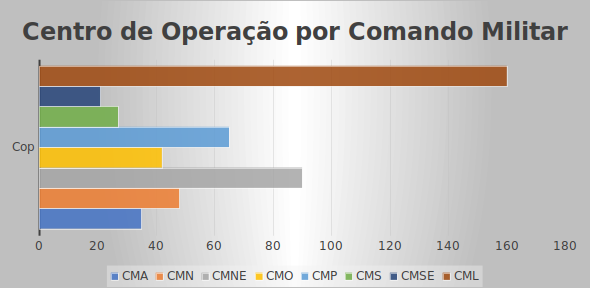
\includegraphics[width=1\textwidth]{Figuras/qtde2_cops.png}
        \caption{Gráfico de COps por Comandos Militar.}
        \label{figuraCops}
\end{figure}

% \hspace{1.5cm}
\textbf{Tabela \ref{QuantidadeAgentes}} É apresentado a distribuição de frequências do número de Agente numa amostra dos Comando Militar de Área do Exército Brasileiro. 

% Agentes
\begin{table}[H]
\centering
\begin{tabular}{|c | c| c|} 
 \multicolumn{3}{c}{Agente por Comando Militar}\\ \hline
  Comando Militar & freq  & percentagem \\ [0.5ex] 
 \hline
 Comando Militar da Amazônia (CMA) &  1224 & 4,88\\ 
 \hline
 Comando Militar do Norte (CMN) &  1496 & 5,97\\
 \hline
 Comando Militar do Nordeste (CMNE) &  4350 & 17,36\\
 \hline
 Comando Militar do Oeste (CMO) &  336 & 1,34\\
 \hline
 Comando Militar do Planalto (CMP) &  1026 & 4,09\\
 \hline
 Comando Militar do Sul (CMS) &  350 & 1,40\\
 \hline
 Comando Militar do Sudeste (CMSE) &  2196 & 8,76\\
 \hline
 Comando Militar do Leste (CML) &  14082 & 56,19\\ [1ex] 
 \hline
\end{tabular}
\caption{Quantidade de Agentes por Comando Militar de Área}
\label{QuantidadeAgentes}
\end{table}

% \hspace{1.5cm}
A representação gráfica da distribuição de frequência dos Agentes é dada pelo gráfico \ref{figuraAgentes}.
\begin{figure}[H]
        \centering
        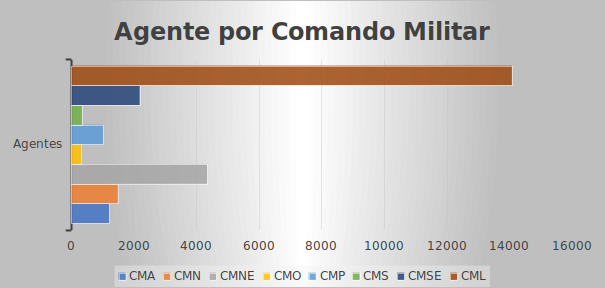
\includegraphics[width=1\textwidth]{Figuras/qtde_agentes.png}
        \caption{Gráfico de Agentes por Comandos Militar.}
        \label{figuraAgentes}
\end{figure}

% \hspace{1.5cm}
\textbf{Tabela \ref{QuantidadeIncidentes}} É apresentado a distribuição de frequências do número de Incidente numa amostra dos Comando Militar de Área do Exército Brasileiro. 
% Incidentes
\begin{table}[H]
\centering
\begin{tabular}{|c | c| c|} 
 \multicolumn{3}{c}{Incidente por Comando Militar}\\ \hline
  Comando Militar & freq   & percentagem \\ [0.5ex] 
 \hline
 Comando Militar da Amazônia (CMA) & 2280 & 21,80\\ 
 \hline
 Comando Militar do Norte (CMN) &  2301 & 22,00\\
 \hline
 Comando Militar do Nordeste (CMNE) &  3774 & 36,09\\
 \hline
 Comando Militar do Oeste (CMO) & 259 & 2,48\\
 \hline
 Comando Militar do Planalto (CMP) &  154 & 1,47\\
 \hline
 Comando Militar do Sul (CMS) &  203 & 1,94\\
 \hline
 Comando Militar do Sudeste (CMSE) &  79 & 0,76\\
 \hline
 Comando Militar do Leste (CML) &  1407 & 13,46\\ [1ex] 
 \hline
\end{tabular}
\caption{Quantidade de Incidentes por Comando Militar de Área}
\label{QuantidadeIncidentes}
\end{table}

% \hspace{1.5cm}
A representação gráfica da distribuição de frequência dos Incidentes é dada pelo gráfico \ref{figuraIncidentes}.
\begin{figure}[H]
        \centering
        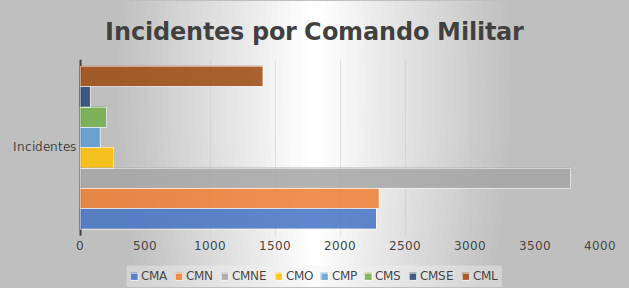
\includegraphics[width=1\textwidth]{Figuras/qtde_incidentes.png}
        \caption{Gráfico de Incidentes por Comandos Militar.}
        \label{figuraIncidentes}
\end{figure}

% \hspace{1.5cm}
\textbf{Tabela \ref{QuantidadeAcoes}} É apresentado a distribuição de frequências do número de Ação numa amostra dos Comando Militar de Área do Exército Brasileiro. 
% Ações
\begin{table}[H]
\centering
\begin{tabular}{|c | c| c|} 
 \multicolumn{3}{c}{Ação por Comando Militar}\\ \hline
  Comando Militar & freq   & percentagem \\ [0.5ex] 
 \hline
 Comando Militar da Amazônia (CMA) &  3193 & 22,22\\ 
 \hline
 Comando Militar do Norte (CMN) &  572 & 3,98\\
 \hline
 Comando Militar do Nordeste (CMNE) &  3009 & 20,94\\
 \hline
 Comando Militar do Oeste (CMO) &  3444 & 23,97\\
 \hline
 Comando Militar do Planalto (CMP) &  1031 & 7,18\\
 \hline
 Comando Militar do Sul (CMS) &  190 & 1,32\\
 \hline
 Comando Militar do Sudeste (CMSE) &  842 & 5,86\\
 \hline
 Comando Militar do Leste (CML) &  2087 & 14,53\\ [1ex] 
 \hline
\end{tabular}
\caption{Quantidade de Ações por Comando Militar de Área}
\label{QuantidadeAcoes}
\end{table}

% \hspace{1.5cm}
A representação gráfica da distribuição de frequência dos Ações é dada pelo gráfico \ref{figuraAcoes}.
\begin{figure}[H]
        \centering
        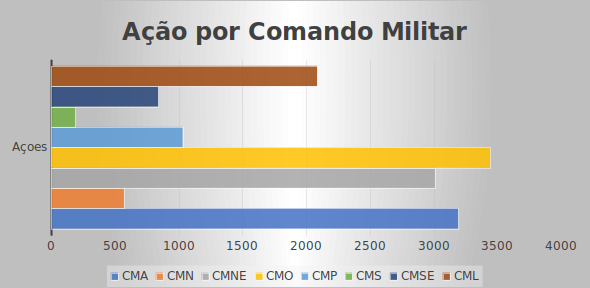
\includegraphics[width=1\textwidth]{Figuras/qtde_acoes.png}
        \caption{Gráfico de Ações por Comandos Militar.}
        \label{figuraAcoes}
\end{figure}

% \hspace{1.5cm}
\textbf{Tabela \ref{QuantidadeRelatos}} É apresentado a distribuição de frequências do número de Relato numa amostra dos Comando Militar de Área do Exército Brasileiro. 
% Relatos
\begin{table}[H]
\centering
\begin{tabular}{|c | c| c|} 
 \multicolumn{3}{c}{Relato por Comando Militar}\\ \hline
  Comando Militar & freq  & percentagem  \\ [0.5ex] 
 \hline
 Comando Militar da Amazônia (CMA) &  259 & 5,53\\ 
 \hline
 Comando Militar do Norte (CMN) &  371 & 7,93\\
 \hline
 Comando Militar do Nordeste (CMNE) &  1334 & 28,50\\
 \hline
 Comando Militar do Oeste (CMO) &  15 & 0,32\\
 \hline
 Comando Militar do Planalto (CMP) &  158 & 3,38\\
 \hline
 Comando Militar do Sul (CMS) &  611 & 13,06\\
 \hline
 Comando Militar do Sudeste (CMSE) &  1476 & 31,54\\
 \hline
 Comando Militar do Leste (CML) &  456 & 9,74\\ [1ex] 
 \hline
\end{tabular}
\caption{Quantidade de Relatos por Comando Militar de Área}
\label{QuantidadeRelatos}
\end{table}

% \hspace{1.5cm}
A representação gráfica da distribuição de frequência dos Relatos é dada pelo gráfico \ref{figuraRelatos}.
\begin{figure}[H]
        \centering
        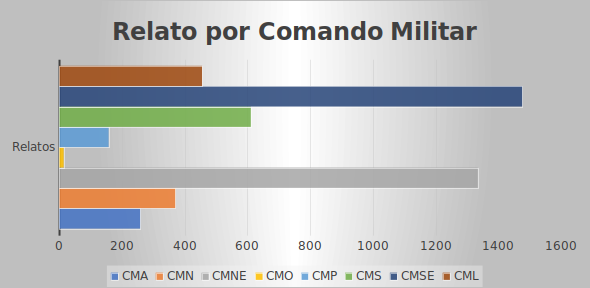
\includegraphics[width=1\textwidth]{Figuras/qtde_relatos.png}
        \caption{Gráfico de Relatos por Comandos Militar.}
        \label{figuraRelatos}
\end{figure}

%\hspace{1.5cm}
%\textbf{Tabela \ref{QuantidadeKmls}} É apresentado a distribuição de frequências do número de Kml numa amostra dos Comando Militar de Área do Exército Brasileiro. 
% Kmls
% \begin{table}[H]
% \centering
% \begin{tabular}{|c | c| c|} 
%  \multicolumn{3}{c}{Kml por Comando Militar}\\ \hline
%   Comando Militar & freq  & percentagem  \\ [0.5ex] 
%  \hline
%  Comando Militar da Amazônia (CMA) &  40 & 11,17\\ 
%  \hline
%  Comando Militar do Norte (CMN) &  21 & 5,87\\
%  \hline
%  Comando Militar do Nordeste (CMNE) &  92 & 25,70\\
%  \hline
%  Comando Militar do Oeste (CMO) &  18 & 5,03\\
%  \hline
%  Comando Militar do Planalto (CMP) &  40 & 11,17\\
%  \hline
%  Comando Militar do Sul (CMS) &  4 & 1,12\\
%  \hline
%  Comando Militar do Sudeste (CMSE) &  14 & 3,91\\
%  \hline
%  Comando Militar do Leste (CML) &  129 & 36,03\\ [1ex] 
%  \hline
% \end{tabular}
% \caption{Quantidade de Kmls por Comando Militar de Área}
% \label{QuantidadeKmls}
% \end{table}

%\hspace{1.5cm}
%A representação gráfica da distribuição de frequência dos Kmls é dada pelo gráfico \ref{figuraKmls}
% \begin{figure}[H]
%         \centering
%         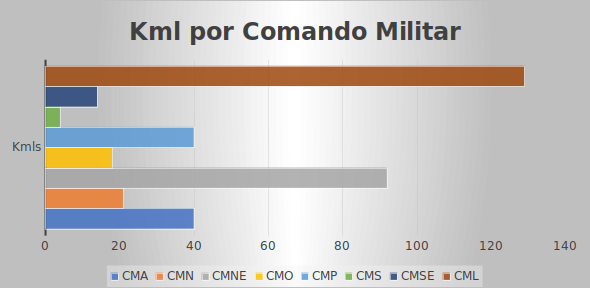
\includegraphics[width=1\textwidth]{Figuras/qtde_kmls.png}
%         \caption{Gráfico de Kmls por Comandos Militar.}
%         \label{figuraKmls}
% \end{figure}

% \hspace{1.5cm}
\textbf{Tabela \ref{QuantidadePois}} É apresentado a distribuição de frequências do número de Ponto de referência (POI) numa amostra dos Comando Militar de Área do Exército Brasileiro. 
% Pois
\begin{table}[H]
\centering
\begin{tabular}{|c | c| c|} 
 \multicolumn{3}{c}{Ponto de Interesse Operação por Comando Militar}\\ \hline
  Comando Militar & freq  & percentagem  \\ [0.5ex] 
 \hline
 Comando Militar da Amazônia (CMA) &  373 & \\ 
 \hline
 Comando Militar do Norte (CMN) &  61 & 3,44\\
 \hline
 Comando Militar do Nordeste (CMNE) &  357 & 20,16\\
 \hline
 Comando Militar do Oeste (CMO) &  14 & 0,79\\
 \hline
 Comando Militar do Planalto (CMP) &  55 & 3,11\\
 \hline
 Comando Militar do Sul (CMS) &  117 & 6,61\\
 \hline
 Comando Militar do Sudeste (CMSE) &  137 & 7,74\\
 \hline
 Comando Militar do Leste (CML) &  657 & 37,10\\ [1ex] 
 \hline
\end{tabular}
\caption{Quantidade de Ponto de interesse por Comando Militar de Área}
\label{QuantidadePois}
\end{table}

% \hspace{1.5cm}
A representação gráfica da distribuição de frequência dos COps é dada pelo gráfico \ref{figuraPois}
\begin{figure}[H]
        \centering
        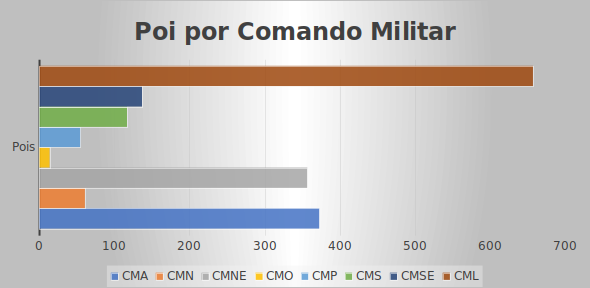
\includegraphics[width=1\textwidth]{Figuras/qtde_pois.png}
        \caption{Gráfico de Pontos de interesse por Comandos Militar.}
        \label{figuraPois}
\end{figure}

% \hspace{1.5cm}
Através do modelo de análise proposto, é possível verificar, tabela \ref{QuantidadeAgentes}. que no CML - Comando Militar do Leste, a utilização de agentes possui uma frequência superior aos demais comandos, devido as intervenções militares e as diversas atuações do comando na garantia da Lei e da Ordem no referido Estado. É importante destacar que na análise de ações por comando, tabela \ref{QuantidadeAcoes}, observa-se uma utilização substancial no CMO - Comando Militar do Oeste e CMA - Comando Militar da Amazônia, devido as queimadas no centro-oeste e no norte do país em 2019, além do crescente fluxo migratório na região do extremo norte, ocasionando portanto a maior utilização do Sistema Pacificador pelos referidos Comandos Militares. Observando os resultados das tabelas e gráficos percebemos que, através das frequências das variáveis por categoria, a utilização do Sistema de Comando e Controle pelos os Comandos Militares de Área demostra o crescimento da ferramenta Pacificador como reforço aos comandantes, nos diversos níveis, no controle dos elementos que compõem sua Força Tarefa durante um determinado Grande evento, Operações e atividade de Garantia da Lei e Ordem. 
 


% % Instituto Federal de Educação, Ciência e Tecnologia Baiano - Campus Guanambi
% 
% Modelo para Trabalho de Conclusão de Curso em LaTeX
% Superior de Análise e Desenvolvimento de Sistemas
% Alterado por: Dr. Naidson Clayr Santos Ferreira
%
% ----------------------------------------------------------------------- %
% Arquivo: definicao-problema.tex
% ----------------------------------------------------------------------- %

% DEFINIÇÃO DO PROBLEMA--------------------------------------------------------

\chapter{DEFINIÇÃO DO PROBLEMA}
\label{chap:definicaoproblema}

No ano de 2012 aconteceu no Brasil a Rio+20, Conferência das Nações Unidas sob o Meio Ambiente. Este seria um grande evento onde a questão segurança foi delegada ao Exército Brasileiro, no tocante a coordenação, preparo e emprego das Forças Federais, Estaduais e Municipais. Com este ambiente operacional foi criado um sistema de Comando e Controle, com vista a auxiliar os comandantes na tarefa de realizar a gerencia ações, para que a Conferencia ocorresse da melhor forma possível. Até os dias atuais este sistema vêm sendo utilizados nos diversos Comando de Área, buscando ser uma ferramenta de auxílio nas demandas operacionais. 

Dentro deste contexto operacional e das complexidades do teatro de operações, como o sistema de comando e controle Pacificador auxilia no apoio a decisão. Portanto, um estudo aprofundado no quesito é necessário para que sejam analisadas as utilizações do sistema \textit{Pacificador}, no auxilio aos comandantes nas diversas operações em todo Territórios Nacional, seja nos grandes eventos (FIFA 2014, Olimpíadas...) ou nas operações de GLO, até os dias atuais.

% as dificuldades envolvidas no ensino de programação em certas instituições, por se tratar de um problema de interesse comum, o que poderá, até mesmo, contribuir com processos que englobam temas socioeconômicos regionais inseridos na realidade de cada instituição, além de apresentar relevante valor para o meio acadêmico.


% O Problema de pesquisa é um questão específica que você quer investigar dentro do seu tema. Uma questão que pode e mereça ser investigada.

% Se o seu tema é logística, por exemplo, para desenvolver o seu TCC, você tem que definir uma questão específica que você quer investigar dentro da logística, do tipo: gestão de estoques e competitividade, custos de transportes… e por aí vai.

% E isso vale para qualquer área do conhecimento. Se o seu tema é Direito do Trabalho, para fazer um TCC, você precisa definir que questão específica quer investigar dentro das possibilidades do Direito do Trabalho. Talvez um ordenamento jurídico específico, por exemplo. Se o seu tema é educação infantil, você também precisa escolher uma questão específica que quer investigar nessa área. E isso vale para Medicina, Serviço Social, Odontologia… e para qualquer área de conhecimento.



% 
\chapter{REFERENCIAIS TEÓRICOS}
\label{chap:refenciaisteoricos}

Segundo \citeonline{comandoecontrole2015} com o expresso uso de tecnologia nos combates modernos, devido a presença de civis, meios de difusão de informações no ambiente operacional. O outro fator é a necessidade de um  sistema de combate com maior proteção coletiva, velocidade e letalidade seletiva. Para tal fim, as ações de comando se desenrolam em todos seus estágios, até o cumprimento das mesma. O comandante, dentro desta linha, poderá consignar novas ordens, para melhor evolução da situação em determinada operação.

Para \citeonline{undestanding2006} nos dias de hoje as missões são ao mesmo tempo mais complexas e dinâmicas, onde requerem maior capacidade coletiva e organização muito mais efetiva para um maior sucesso operacional. O avanço da  Tecnologia de Informação vem criando um novo espaço onde organizações e indivíduos possam operar aprendendo a tomar vantagens sobre as oportunidades oferecidas nas operações sub-saindo aqueles que as ignoraram.


Ainda para \citeonline{comandoecontrole2015} O procedimento decisório envolve a obtenção de dados, a reunião de fatores intervenientes, o conhecimento da consciência situacional, até a decisão final. Nessa perspectiva, a ação de Comando e Controle (C2) é relevante ao triunfo nas diversas missões operacionais. Sua concepção se dá através de métodos, procedimentos, características  e vocabulários pecuniários de forma sistêmica. Nos dias atuais as decisões, dentro deste ambiente operacional, ficaram cada vez mais submetidas aos Sistemas de Tecnologia da Informação e Comunicações (TIC) no auxilio das execuções de comando e controle de forma rápida, efetiva e precisa. Os combates modernos têm nos sistemas de TIC todas as suas atividades operacionais e de apoio auxiliando o comandante, nos diversos níveis, suas decisões, com maior rapidez, análise, difusão dos conhecimentos para todos os escalões. Isto tudo busca uma melhor atividade operacional de comando e controle na incumbência da vitória. 





% % Instituto Federal de Educação, Ciência e Tecnologia Baiano - Campus Guanambi
% 
% Modelo para Trabalho de Conclusão de Curso em LaTeX
% Superior de Análise e Desenvolvimento de Sistemas
% Alterado por: Dr. Naidson Clayr Santos Ferreira
%
% ----------------------------------------------------------------------- %
% Arquivo: justificativa.tex
% ----------------------------------------------------------------------- %

% JUSTIFICATIVA-----------------------------------------------------------------

\chapter{JUSTIFICATIVA}
\label{chap:justificativa}
O pacificador é uma ferramenta relativamente nova no EB e que é testada cada vez que acontece algum grande evento, ou seja, é na prática que ele é testado e aprovado ou reprovado em alguns quesitos, dessa forma, acreditamos que realizar um levantamento estatístico ajudaria a sua equipe de desenvolvedores entender alguns gargalos e prováveis falhas que poderiam ser acertadas, assim como, confirmar tudo aquilo que tem funcionado muito bem ao longo desses anos.
Esta maturidade somente pode ser obtida, com a confirmação que suas funcionalidades estão atendendo perfeitamente às necessidades da Força Terrestre e de todos os órgãos envolvidos nos mais variados eventos em que o pacificador é utilizado, e isso no nosso entender avaliza uma análise qualitativa e quantitativa sobre suas funcionalidades, quais solicitações são mais comuns, quais solicitações ficam sem ser atendidas ou atendidas em parte, quais os logs de erros mais comuns na ferramenta.

Devidamente autorizados a ter acesso aos dados salvos em seus servidores e com o único fim de realizar este estudo, e sem identificar cada grande evento, estudaremos cada área que entendermos ser importante relatar e coletaremos a informação proveitosa à nossa pesquisa, sendo assim, acreditamos que ao longo do estudo devam surgir outros questionamentos ou até informações que podem ser de grande relevância ao que está proposto nesse tópico.

% No Brasil, segundo \citeonline{gomes2008proposta}, \citeonline{doslinguagem} e \citeonline{junior2005ensino}, as disciplinas de algoritmo e programação são responsáveis tanto por um grande número de reprovações como também representam uma das causas da evasão de estudantes em cursos de computação no ensino superior e médio/técnico em instituições públicas. Tal fato pode estar relacionado ao nível teórico do material estudado uma vez que a programação possui conceitos próprios e, de certa forma, pouco compartilhados com as demais disciplinas, sua especificidade nos módulos iniciais bem como a não difusão do contexto nas escolas públicas de ensino básico nos anos anteriores.

% De acordo com \citeonline{manhaes2011previsao}, diversos fatores podem ser apontados como possíveis causas de evasão de alunos, entre eles é possível reconhecer aspectos socioeconômicos regionais, localização geográfica, tempo de duração e adequação ao mercado de trabalho. Isso significa que suas principais causas podem variar entre instituições e regiões específicas e, por se tratar de um componente curricular de significância maior dentro de um curso de computação, as causas de seu elevado número de reprovações e evasões devem ser melhor estudadas e analisadas para que se possa criar indicadores capazes de determinar as principais fontes do problema.
%Na Justificativa deve-se mostrar, com fatos e argumentos, porque o projeto é importante e deve ser desenvolvido. Quais fatos, ideias ou leituras mostram que o tema precisa ser estudado? Qual a relevância do tema? Também é necessário pensar de qual Linha de Pesquisa do TC o projeto estaria mais próximo.

%Para tal, discussão mais aprofundada se torna necessária a fim de demonstrar como isso pode vir a atingir o ensino, não apenas em determinada instituição mas, também, dentro de um contexto social. É necessário que se discuta suas causas e consequências e como elas se relacionam para que, até mesmo, seus professores tenham melhor ideia de como lidar com esse quesito, sem que haja perda no desempenho dos alunos ou até dos próprios professores, beneficiando a instituição e sociedade ao final desse processo. Por outro lado, negar a existência do problema em questão, ignorando sua origem e efeitos, bem como a importância da discussão do tema poderá representar um esgotamento no curso de computação com rapidez proporcional ao nível de evasão dos estudantes.

%Portanto, um estudo aprofundado no quesito é necessário para que sejam analisadas as dificuldades envolvidas no ensino de programação em certas instituições, por se tratar de um problema de interesse comum, o que poderá, até mesmo, contribuir com processos que englobam temas socioeconômicos regionais inseridos na realidade de cada instituição, além de apresentar relevante valor para o meio acadêmico. 

     

% % Instituto Federal de Educação, Ciência e Tecnologia Baiano - Campus Guanambi
% 
% Modelo para Trabalho de Conclusão de Curso em LaTeX
% Superior de Análise e Desenvolvimento de Sistemas
% Alterado por: Dr. Naidson Clayr Santos Ferreira
%
% ----------------------------------------------------------------------- %
% Arquivo: Objetivo Geral.tex
% ----------------------------------------------------------------------- %

% OBJETIVOS-------------------------------------------------------------------

\chapter{OBJETIVOS}
\label{chap:objetivos}

\section{Objetivo Geral}
\label{sec:objetivogeral}

Realizar o levantamento qualitativo e quantitativo dos dados mais relevantes que sejam atinentes à parte operacional do Pacificador para tentar entender quais os incidentes mais comuns, média de tempo de resolução dos incidentes ao longo dos anos, quantas e quais operações o sistema já apoiou, quantidade de usuários que utilizaram o sistema e quais os Centros de Operações foram criados ao longo dos anos de existência do Pacificador.
%Identificar, através da mineração de dados, as possíveis causas de reprovação e evasão, bem como analisar os principais fatores que  determinam o desempenho de alunos em disciplinas de algoritmo e programação nos cursos superiores e técnicos de informática, para que seja possível examinar suas principais origens dentro do contexto educacional.  

\section{Objetivos Específicos}
\label{sec:objetivosespecificos}

\begin{itemize}
    \item Indicar métodos utilizados na coleta de dados que possibilitem a análise qualitativa e quantitativa  da ferramenta;
    \item Identificar as causas mais comuns que dificultam e atrasam a resolução dos incidentes;
    \item Levantar quantas e em quais Operações o Pacificador já foi utilizado;
    \item Sugerir quais melhorias podem ser realizadas para refinar mais a utilização por parte dos usuários melhorando assim a resposta para os tomadores de decisão.
\end{itemize}

% \include{estrutura/textuais/desenvolvimento/revisao-bibliografica-teorica} 

% \chapter{METODOLOGIA}
\label{chap:metodologia}

Aspirando solucionar o problema de pesquisa levantado e detalhar o caminho a ser percorrido durante a pesquisa exploratória, para alcançar o objetivo do presente trabalho. A fim de delineação de pesquisa foi considerado as fases de levantamento e seleção da bibliografia, coleta de dados, critica dos dados, leitura analítica e fichamento das fontes, obtenção dos dados no sistema Pacificados, argumentação e discussão dos resultados.

As revisões de literaturas, sob o termo de interesse, será realizado uma busca, em Português e Inglês, nas seguintes fontes de busca:
\begin{itemize}
    \item Artigos  disponíveis  nos  anais do International  Command  and  Control  Research and  Technology  Symposium(ICCRTS),  organizado  anualmente  pelo  Departamento  de Defesa Americano;
    \item Artigos  científicos  indexados  no  Portal  de  Periódicos  da  Coordenação  de Aperfeiçoamento de Pessoal de Nível Superior (CAPES);
    \item Documentação  de  grupos  de  trabalho  relacionados  da  OTAN(Organização  do Tratado do Atlântico Norte);
    \item Documentação  de  grupos  de  trabalho  relacionados  da  OTAN(Organização  do Tratado do Atlântico Norte);
    \item Manuais de Campanha.
\end{itemize}

O presente estudo identifica-se como uma pesquisa do tipo exploratória com vista a avaliar o desempenho do sistema de comando e controle \textit{Pacificador}, nas operações.                	 

% \include{estrutura/textuais/desenvolvimento/resultadosesperados}       	  

% \chapter{METODOLOGIA}
\label{chap:metodologia}

Aspirando solucionar o problema de pesquisa levantado e detalhar o caminho a ser percorrido durante a pesquisa exploratória, para alcançar o objetivo do presente trabalho. A fim de delineação de pesquisa foi considerado as fases de levantamento e seleção da bibliografia, coleta de dados, critica dos dados, leitura analítica e fichamento das fontes, obtenção dos dados no sistema Pacificados, argumentação e discussão dos resultados.

As revisões de literaturas, sob o termo de interesse, será realizado uma busca, em Português e Inglês, nas seguintes fontes de busca:
\begin{itemize}
    \item Artigos  disponíveis  nos  anais do International  Command  and  Control  Research and  Technology  Symposium(ICCRTS),  organizado  anualmente  pelo  Departamento  de Defesa Americano;
    \item Artigos  científicos  indexados  no  Portal  de  Periódicos  da  Coordenação  de Aperfeiçoamento de Pessoal de Nível Superior (CAPES);
    \item Documentação  de  grupos  de  trabalho  relacionados  da  OTAN(Organização  do Tratado do Atlântico Norte);
    \item Documentação  de  grupos  de  trabalho  relacionados  da  OTAN(Organização  do Tratado do Atlântico Norte);
    \item Manuais de Campanha.
\end{itemize}

O presente estudo identifica-se como uma pesquisa do tipo exploratória com vista a avaliar o desempenho do sistema de comando e controle \textit{Pacificador}, nas operações.               
% Instituto Federal de Educação, Ciência e Tecnologia Baiano - Campus Guanambi
% 
% Modelo para Trabalho de Conclusão de Curso em LaTeX
% Superior de Análise e Desenvolvimento de Sistemas
% Alterado por: Dr. Naidson Clayr Santos Ferreira
%
% ----------------------------------------------------------------------- %
% Arquivo: conclusao.tex
% ----------------------------------------------------------------------- %

% CONCLUSÃO--------------------------------------------------------------------

\chapter{CONCLUSÃO}
\label{chap:conclusao}

O Exército Brasileiro tem um papel importante nos mais variados cenários do Estado Brasileiro, seja na ajuda humanitária da operação pipa no Nordeste, ou nas catástrofes como as que vem acontecendo ao longo do ano de 2019, as quais podemos citar operação contra incêndios na Amazônia brasileira e limpeza do óleo nas praias da Região Nordeste, além disso, podemos citar intervenção federal no Estado do Rio de Janeiro, entre tantas outras operações realizadas pela força terrestre em território nacional e até mesmo internacional nas operações de paz.
Vivemos um momento sem precedentes na história da segurança pública, onde o crime organizado se vale de tecnologia para realizar o planejamento de suas ações, além de ter armamentos e equipamentos com alto poder de dissuasão. É neste contexto que o Pacificador Web é inserido, com o objetivo de apoiar à decisão dos comandantes das mais variadas operações trazendo todo tipo de informação relevante sobre o terreno, status dos amigos e inimigos entre tantas informações necessárias para o cumprimento da missão. 
Entendemos que o Pacificador Web é uma excelente ferramenta que se adequa a qualquer uma das operações que o Exército executa no momento, tanto que já foi testado e aprovado inúmeras vezes nas mais variadas operações desde a Conferência das Nações Unidas (Rio +20) em 2012 até as operações que estão sendo executadas neste momento.
Vimos que um importante “gargalo” na utilização do Pacificador é a dependência pela telefonia móvel, que é gerenciada por empresas privadas de telefonia e que nem sempre têm uma cobertura de sinal satisfatória nas localidades onde as operações se desenvolvem. Dessa maneira, entendemos que poderia ser encontrado um meio mais seguro de interligação entre os dispositivos móveis e os servidores, como uma rede via satélite.
Analisando os dados no período compreendido entre janeiro de 2017 até outubro de 2019, vimos que a maioria dos Centros de Operações estão lotados no Comando Militar do Leste (CML) com mais de 32 por cento da totalidade de todo o território nacional, sendo que o Comando Militar do Sudeste (CMSE) é o que tem menos Centros de Operações com 4 por cento. Isto comprova que o CML no momento é o C Mil A que mais utiliza o Pacificador, além de ser o Comando que mais tem operações de GLO, no período escolhido para análise.
Na avaliação que fizemos no número de Agentes por C Mil A, o CML ainda pontua como o que tem mais agentes com mais de 14 mil agentes, enquanto o CMS que é considerado o maior C Mil A tem apenas 350 agentes no período da análise.
Já na tabela 3 identificamos um aumento de incidentes significativo no CMA e CMNE o que leva a crermos que o Pacificador foi amplamente utilizado na Operação Acolhida e nas operações de combate ao fogo na Amazônia e também nas operações de limpeza do óleo nas praias nordestinas.
O Pacificador é uma realidade no âmbito do Exército, uma ferramenta consolidada que somente precisa manter-se atualizada frente às peculiaridades de cada tipo de operação desenvolvida pelo Exército, dito isso, acreditamos que uma futura pesquisa de campo junto aos agentes que estão nos mais variados teatros de operações, com o intuito da realização de um levantamento de quais funções e atividades precisam ser melhoradas para que este sistema fique o mais adequado o possível, sendo assim citamos uma melhoria que seria a entrada de incidentes e todo tipo de dado seja facilitada pelo a habilitação de reconhecimento de voz o que traria mais segurança aos agentes responsáveis pela entrada de dados.


                 			     
% % Instituto Federal de Educação, Ciência e Tecnologia Baiano - Campus Guanambi
% 
% Modelo para Trabalho de Conclusão de Curso em LaTeX
% Superior de Análise e Desenvolvimento de Sistemas
% Alterado por: Dr. Naidson Clayr Santos Ferreira
%
% ----------------------------------------------------------------------- %
% Arquivo: cronograma.tex
% ----------------------------------------------------------------------- %

% CRONOGRAMA--------------------------------------------------------------------

\chapter{CRONOGRAMA}

Para execução das atividades a serem realizadas até a entrega do Trabalho de Conclusão do Curso (Artigo) teremos as seguintes etapas, conforme \autoref{tab:cronograma} abaixo.

\begin{table}[!ht]
		\centering
		\caption{Cronograma de Atividades - Semestre II-2019}
\Rotatebox{90}{%
\scalebox{0.65}{
\begin{tabular}{lcccccccccc}
\rowcolor[HTML]{C0C0C0} 
\hline
\multicolumn{1}{c}{\cellcolor[HTML]{C0C0C0}}                                     & \multicolumn{8}{c}{\cellcolor[HTML]{C0C0C0}\textbf{Período}}                                                                                       \\
\rowcolor[HTML]{C0C0C0} 
\multicolumn{1}{c}{\cellcolor[HTML]{C0C0C0}}                                     & \multicolumn{8}{c}{\cellcolor[HTML]{C0C0C0}\textbf{II Semestre de 2019}} 
\\
\rowcolor[HTML]{C0C0C0} 
\multicolumn{1}{c}{\multirow{-3}{*}{\cellcolor[HTML]{C0C0C0}\textbf{Atividade}}} & \textbf{29/7 a} & \textbf{3/8 a} & \textbf{26/8 a} & \textbf{31/8 a} & \textbf{7/9 a}  & \textbf{21/9 a} & \textbf{25/9 a} &

\\
\rowcolor[HTML]{C0C0C0} 
\multicolumn{1}{c}{\multirow{-3}{*}{\cellcolor[HTML]{C0C0C0}\textbf{}}} & \textbf{2/8/2019} & \textbf{25/8/2019} & \textbf{30/8/2019} & \textbf{6/9/2019} & \textbf{20/9/2019}  & \textbf{24/9/2019} & \textbf{30/9/2019} &

\\
\hline
Escolha do Tema                            & \textbf{$\bullet$}   & \textbf{}   & \textbf{}   & \textbf{}    & \textbf{}     & \textbf{}    & \textbf{} & \\
\rowcolor[HTML]{EFEFEF} 
Definição do Tema, Introdução, Objetivos e Problema                             & \textbf{}   & \textbf{$\bullet$}   & \textbf{$\bullet$}   & \textbf{}    & \textbf{}  & \textbf{} & \textbf{}      &        \\
% \rowcolor[HTML]{EFEFEF} 
Elaboração da Justificativa e Hipóteses                                          & \textbf{}    & \textbf{$\bullet$}   & \textbf{$\bullet$}   & \textbf{}    & \textbf{} & \textbf{} & \textbf{} &\\
\rowcolor[HTML]{EFEFEF}
Elaboração dos Instrumentos de Coleta de Dados
                                     & \textbf{}    & \textbf{}   & \textbf{}   & \textbf{$\bullet$}    & \textbf{} & \textbf{} & \textbf{} &\\
Coleta de dados                                          & \textbf{}    & \textbf{}   & \textbf{}   & \textbf{}    & \textbf{$\bullet$} & \textbf{} & \textbf{} &\\
\rowcolor[HTML]{EFEFEF}
Análise dos dados                                          & \textbf{}    & \textbf{}   & \textbf{}   & \textbf{}    & \textbf{$\bullet$} & \textbf{} & \textbf{} &\\
Redação do Artigo científico                                          & \textbf{}    & \textbf{}   & \textbf{}   & \textbf{}    & \textbf{} & \textbf{$\bullet$} & \textbf{} &\\
\rowcolor[HTML]{EFEFEF}
Revisão e redação final                                          & \textbf{}    & \textbf{}   & \textbf{}   & \textbf{}    & \textbf{} & \textbf{} & \textbf{$\bullet$} &\\
Entrega do artigo científico                                          & \textbf{}    & \textbf{}   & \textbf{}   & \textbf{}    & \textbf{} & \textbf{} & \textbf{$\bullet$} &\\
% Definição do Tema, Introdução, Objetivos e Problema                             & \textbf{$\bullet$}   & \textbf{$\bullet$}   & \textbf{}   & \textbf{}    & \textbf{}                \\
% \rowcolor[HTML]{EFEFEF} 
% Elaboração da Justificativa e Hipóteses                                          & \textbf{$\bullet$}    & \textbf{$\bullet$}   & \textbf{}   & \textbf{}    & \textbf{} &\\
% Revisão Bibliográfica / Teórica da pesquisa                                      & \textbf{$\bullet$}    & \textbf{$\bullet$}   & \textbf{}   & \textbf{}   & \textbf{} &\\
% \rowcolor[HTML]{EFEFEF} 
% Definição da Metodologia                                                         & \textbf{$\bullet$}    & \textbf{$\bullet$}    & \textbf{}   & \textbf{}   & \textbf{} &\\
% Elaboração dos Instrumentos de Coleta de Dados                                   & \textbf{}    & \textbf{$\bullet$}    & \textbf{$\bullet$}   & \textbf{$\bullet$}   & \textbf{} &\\
% \rowcolor[HTML]{EFEFEF} 
% Coleta dos dados da pesquisa                                                               & \textbf{}    & \textbf{$\bullet$}    & \textbf{$\bullet$}    & \textbf{$\bullet$}   & \textbf{} &\\
% Análise dos dados da pesquisa                                                               & \textbf{}    & \textbf{$\bullet$}    & \textbf{$\bullet$}    & \textbf{$\bullet$}   & \textbf{} &\\
% \rowcolor[HTML]{EFEFEF} 
% Defesa do Pré-TCC                                                                & \textbf{}    & \textbf{}    & \textbf{}    & \textbf{}    & \textbf{$\bullet$}     &              &              \\
% Realização da Pesquisa                                                           & \textbf{}    & \textbf{}    & \textbf{}    & \textbf{}    & \textbf{$\bullet$}      &              &              \\
% \rowcolor[HTML]{EFEFEF} 
% Coleta dos dados da pesquisa                                                     &              &              &              &              & \textbf{}    & \textbf{}    & \textbf{}    & \textbf{$\bullet$}   & \textbf{$\bullet$}   & \textbf{}    \\
% Análise dos dados da pesquisa                                                    &              &              &              &              & \textbf{}    & \textbf{}    & \textbf{}    & \textbf{$\bullet$}   & \textbf{$\bullet$}   & \textbf{}    \\
% \rowcolor[HTML]{EFEFEF} 
% Revisão do Pré-TCC e Elaboração do TCC                                           &              &              &              &              & \textbf{}    & \textbf{}    & \textbf{}    & \textbf{}    & \textbf{$\bullet$}   & \textbf{$\bullet$}   \\
% Entrega do TCC                                                                   &              &              &              &              & \textbf{}    & \textbf{}    & \textbf{}    & \textbf{}    & \textbf{$\bullet$}   & \textbf{$\bullet$}   \\
% \rowcolor[HTML]{EFEFEF} 
% Defesa do TCC & & & & & \textbf{} & \textbf{} & \textbf{} & \textbf{} & \textbf{} & \textbf{$\bullet$}\\
\hline

\end{tabular}
}
}
\fonte Própria (2019).
		\label{tab:cronograma}
\end{table} 								  

\postextual
% INSERE ELEMENTOS PÓS-TEXTUAIS
% Instituto Federal de Educação, Ciência e Tecnologia Baiano - Campus Guanambi
% 
% Modelo para Trabalho de Conclusão de Curso em LaTeX
% Superior de Análise e Desenvolvimento de Sistemas
% Alterado por: Dr. Naidson Clayr Santos Ferreira
%
% ----------------------------------------------------------------------- %
% Arquivo: referencias.tex
% ----------------------------------------------------------------------- %

% REFERÊNCIAS------------------------------------------------------------------

% Carrega o arquivo "base-referencias.bib" e extrai automaticamente as referências citadas

\bibliography{./base-referencias}
\bibliographystyle{abntex2-alf} % Define o estilo ABNT para formatar a lista de referências
% OBSERVAÇÕES------------------------------------------------------------------
% Este arquivo não precisa ser alterado.
           			       	   % Referências
%% Instituto Federal de Educação, Ciência e Tecnologia Baiano - Campus Guanambi
% 
% Modelo para Trabalho de Conclusão de Curso em LaTeX
% Superior de Análise e Desenvolvimento de Sistemas
% Alterado por: Dr. Naidson Clayr Santos Ferreira
%
% ----------------------------------------------------------------------- %
% Arquivo: apendices.tex
% ----------------------------------------------------------------------- %

% APÊNDICES--------------------------------------------------------------------

\begin{apendicesenv}
\partapendices

% Primeiro apêndice------------------------------------------------------------
\chapter{Nome do apêndice} % Edite para alterar o título deste apêndice
\label{chap:apendiceA}

Lembre-se que a diferença entre apêndice e anexo diz respeito à autoria do texto e/ou material ali colocado.

Caso o material ou texto suplementar ou complementar seja de sua autoria, então ele deverá ser colocado como um apêndice. Porém, caso a autoria seja de terceiros, então o material ou texto deverá ser colocado como anexo.

Caso seja conveniente, podem ser criados outros apêndices para o seu trabalho acadêmico. Basta recortar e colar este trecho neste mesmo documento. Lembre-se de alterar o "label"{} do apêndice.

Não é aconselhável colocar tudo que é complementar em um único apêndice. Organize os apêndices de modo que, em cada um deles, haja um único tipo de conteúdo. Isso facilita a leitura e compreensão para o leitor do trabalho.

% Novo apêndice----------------------------------------------------------------
\chapter{Nome do outro apêndice}
\label{chap:apendiceB}

conteúdo do novo apêndice

\end{apendicesenv}
             			           % Apêndices
%% Instituto Federal de Educação, Ciência e Tecnologia Baiano - Campus Guanambi
% 
% Modelo para Trabalho de Conclusão de Curso em LaTeX
% Superior de Análise e Desenvolvimento de Sistemas
% Alterado por: Dr. Naidson Clayr Santos Ferreira
%
% ----------------------------------------------------------------------- %
% Arquivo: anexos.tex
% ----------------------------------------------------------------------- %

% ANEXO------------------------------------------------------------------------

\begin{anexosenv}
\partanexos

% Primeiro anexo---------------------------------------------------------------
\chapter{Nome do anexo}     % edite para alterar o título deste anexo
\label{chap:anexoA}

Lembre-se que a diferença entre apêndice e anexo diz respeito à autoria do texto e/ou material ali colocado.

Caso o material ou texto suplementar ou complementar seja de sua autoria, então ele deverá ser colocado como um apêndice. Porém, caso a autoria seja de terceiros, então o material ou texto deverá ser colocado como anexo.

Caso seja conveniente, podem ser criados outros anexos para o seu trabalho acadêmico. Basta recortar e colar este trecho neste mesmo documento. Lembre-se de alterar o "label"{} do anexo.

Organize seus anexos de modo a que, em cada um deles, haja um único tipo de conteúdo. Isso facilita a leitura e compreensão para o leitor do trabalho. É para ele que você escreve.

% Novo anexo-------------------------------------------------------------------
\chapter{Nome do outro anexo}
\label{chap:anexoB}

conteúdo do outro anexo

\end{anexosenv}
               			           %   Anexos
%\include{estrutura/textuais/desenvolvimento/orientacoes}                   % Capítulo com Orientações de uso do Template

\end{document}
